\documentclass[tikz,border=12pt]{standalone}
% Shared visual language for standalone EMT block diagrams.
\usepackage{amsmath}
\usetikzlibrary{arrows.meta,backgrounds,calc,fit,positioning}

\tikzset{
    emt diagram/.style = {>={Stealth[length=2.4mm]}},
    line/.style        = {semithick, rounded corners=6pt},
    block/.style       = {draw, semithick, fill=white,
                          minimum height=1cm, minimum width=2.3cm},
    hblock/.style      = {block, minimum width=2.24cm, minimum height=1.3cm},
    vblock/.style      = {block, minimum width=1.3cm, minimum height=2.24cm},
    sum/.style         = {draw, semithick, fill=white, circle,
                          inner sep=2.6pt},
    signal/.style      = {circle, fill, inner sep=1.4pt,
                          label distance=3pt},
    sig/.style         = {font=\small},
    pm/.style          = {font=\scriptsize},
    wire jump/.style   = {line,
                          preaction={draw=white, line width=3pt,
                                     line cap=round}},
    enclosure/.style   = {draw, dashed, semithick, rounded corners=4pt},
    operator enclosure/.style = {enclosure, inner xsep=7mm, inner ysep=6mm}
}


\begin{document}
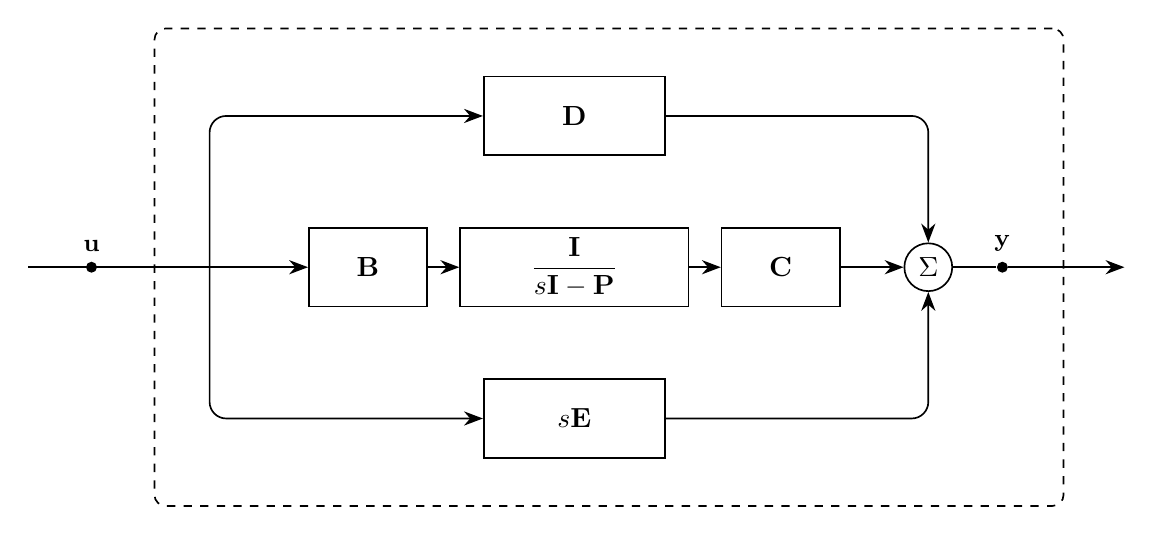
\begin{tikzpicture}[emt diagram]

% State-space chain: input map -> resolvent state bank -> output map
\node[block, minimum width=2.9cm] (res)
    {$\dfrac{\mathbf{I}}{s\mathbf{I} - \mathbf{P}}$};
\node[block, minimum width=1.5cm, left=0.4cm of res] (B) {$\mathbf{B}$};
\node[block, minimum width=1.5cm, right=0.4cm of res] (C) {$\mathbf{C}$};

% Feedthrough paths
\node[block, above=0.9cm of res] (D) {$\mathbf{D}$};
\node[block, below=0.9cm of res] (E) {$s\mathbf{E}$};

% Fan-out from a single internal point
\coordinate (split) at ($(B.west)+(-1.25, 0)$);
\draw[->, line] (split) -- (B.west);
\draw[->, line] (split) |- (D.west);
\draw[->, line] (split) |- (E.west);

% Chain series connections
\draw[->, line] (B.east)   -- (res.west);
\draw[->, line] (res.east) -- (C.west);

% Fan-in to summation
\node[sum, right=0.8cm of C] (S) {$\Sigma$};
\draw[->, line] (C.east) -- (S);
\draw[->, line] (D.east) -| (S.north);
\draw[->, line] (E.east) -| (S.south);

% Input node (owned externally)
\node[signal, label={[sig]above:$\mathbf{u}$}] (uin)
    at ($(split)+(-1.5, 0)$) {};
\draw[line] ($(uin)+(-0.8, 0)$) -- (split);

% Output node (owned by this model) with port arrow out
\node[signal, label={[sig]above:$\mathbf{y}$}, right=0.55cm of S]
    (yout) {};
\draw[line] (S.east) -- (yout);
\draw[->, line] (yout) -- ++(1.55, 0);

% Model enclosure: fixed padding around model-owned paths and output variable
\begin{scope}[on background layer]
    \node[operator enclosure, fit=(split)(B)(res)(C)(D)(E)(S)(yout)] {};
\end{scope}

\end{tikzpicture}
\end{document}
